\documentclass{article}


\usepackage[latin1]{inputenc}
\usepackage{hyperref}
\usepackage{graphicx}
\usepackage{amsmath, amssymb}

%%%%%%%%%%%%%%%% Lengths %%%%%%%%%%%%%%%%
\setlength{\textwidth}{15.5cm}
\setlength{\evensidemargin}{0.5cm}
\setlength{\oddsidemargin}{0.5cm}

%%%%%%%%%%%%%%%% Variables %%%%%%%%%%%%%%%%
\def\projet{5}
\def\titre{Interpolation and integration methods / Cubic splines and surface interpolation}
\def\groupe{2}
\def\equipe{2}
\def\responsible{chelou001}
\def\secretary{desparbes}
\def\others{lgrelet, ndehaiesdit, tagry}

\begin{document}

%%%%%%%%%%%%%%%% Header %%%%%%%%%%%%%%%%
\noindent\begin{minipage}{0.98\textwidth}
  \vskip 0mm
  \noindent
  { \begin{tabular}{p{7.5cm}}
      {\bfseries \sffamily
        Project \projet} \\
      {\itshape \titre}
    \end{tabular}}
  \hfill
  \fbox{\begin{tabular}{l}
      {~\hfill \bfseries \sffamily Group \groupe\ - Team \equipe
        \hfill~} \\[2mm]
      Responsible : \responsible \\
      Secretary : \secretary \\
      Codeurs : \others
    \end{tabular}}
  \vskip 4mm ~

  ~~~\parbox{0.95\textwidth}{\small \textit{Abstract:} \sffamily This project implements a (somewhat basic) model to represent the air flow around an airfoil, i.e. the cross section of an aircraft's wing. The goal consists in obtaining a pressure map above and below the wing, so as to approximate the wing's lift, i.e. its ability to sustain the plane in the air. This is to be done in two steps: first, refine the airfoil into a sufficiently smooth curve, then compute the pressure map using integration methods. }
  \vskip 1mm ~
\end{minipage}

%%%%%%%%%%%%%%%% Main part %%%%%%%%%%%%%%%%
\section{Cubic spline interpolation method}

To obtain an accurate model of air flow, some mathematic tools are needed. First of all, it is necessary to implement an interpolation method. It consists in computing an approximation of a function, based on a finite sample of values taken by this function in known points. In this project, the cubic spline method is chosen: here, the approximation between two consecutive points is a third degree polynom. The continuity of two consecutive polynoms, their derivates and their second derivate is kept to guanrantee the global cohesion of the solution. An interresting choice to compute the cubic spline method is to calculate the second derivate first, and then to deduce the interpolation function itself. The algorithm used in this project is based on an \href{http://www.labri.fr/perso/fpierre/documents_enligne/c3-3.ps}{already-existing code} written in C we adapted to Python. Here is an example of the second derivate of cosinus on $[0, \pi]$ obtained with this algorithm:

\begin{figure}[h]
  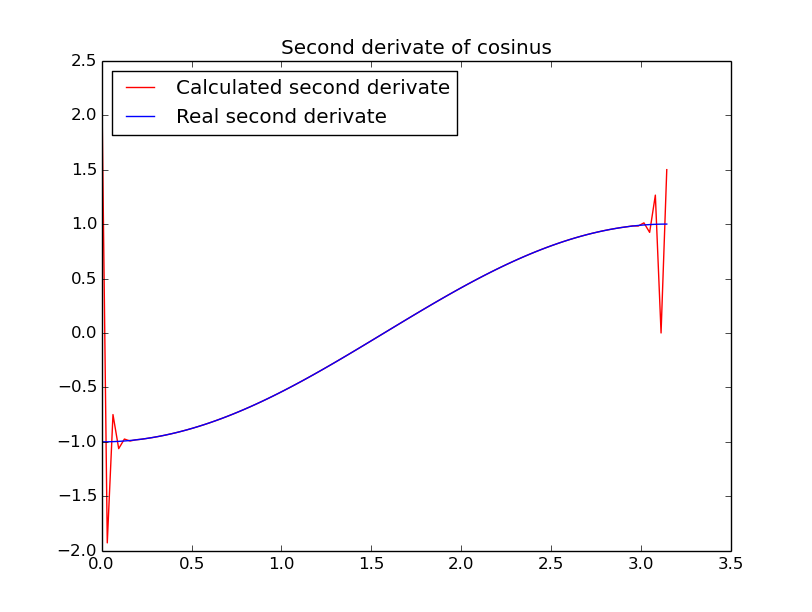
\includegraphics[width=12cm]{cosinus_second_derivate}
\end{figure}

This graph is a comparison between the curve obtained with this algorithm and the real representation of the second derivate of cosinus, which is

\begin{equation}
\begin{array}{ccccl}
\frac{d^2 cos}{dx^2} & : & [0, \pi] & \to & \mathbb{R} \\
 & & x & \mapsto & -cos(x)
\end{array}
\end{equation}

The two curves are similar, but obviously, there are disturbances on each extremity of the computed one. It means that this algorithm sometimes doesn't give a satisfying result for the extreme side values of the considerated interval. This fact will be important for the interpretation of the following results.\\\\

Now that a good approximation of the second derivate of the function is calculated, it is clearly possible to compute the function itself. This is an example of an cubic spline interpolation of cosinus on $[0, \pi]$ :

\begin{figure}[h]
  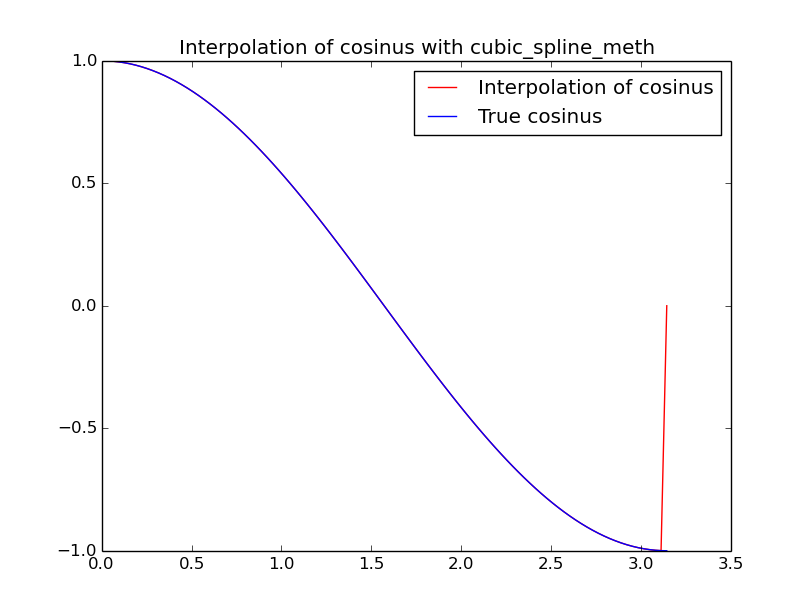
\includegraphics[width=12cm]{cosinus_interpolation}
\end{figure}

\end{document}
